%%%%%%%%%%%%%%%%%%%MAIN_OPTIONS%%%%%%%%%%%%%%%%%%%
\documentclass[a4paper, 14pt]{article}

%% Работа с русским языком
\usepackage{cmap}					% поиск в PDF
\usepackage{hyperref}				% гиперссылки
\usepackage[warn]{mathtext} 		% русские буквы в формулах
\usepackage[T2A]{fontenc}			% кодировка
\usepackage[utf8]{inputenc}			% кодировка исходного текста
\usepackage[english,russian]{babel}	% локализация и переносы

%% Дополнительная работа с математикой
\usepackage{amsfonts,amssymb,amsthm,mathtools} % AMS
\usepackage{amsmath}
\usepackage{icomma} % "Умная" запятая: $0,2$ --- число, $0, 2$ --- перечисление

%% Номера формул
%\mathtoolsset{showonlyrefs=true} % Показывать номера только у тех формул, на которые есть \eqref{} в тексте.

%%FONTS_Packadges
\usepackage{euscript} % Шрифт Евклид
\usepackage{mathrsfs} % Красивый матшрифт

%% Свои команды
\DeclareMathOperator{\sgn}{\mathop{sgn}}

%% Перенос знаков в формулах (по Львовскому)
\newcommand*{\hm}[1]{#1\nobreak\discretionary{}
	{\hbox{$\mathsurround=0pt #1$}}{}}

%%% Работа с картинками
\usepackage{graphicx}  % Для вставки рисунков
\graphicspath{{pictures/}{images2/}}  % папки с картинками
\setlength\fboxsep{3pt} % Отступ рамки \fbox{} от рисунка
\setlength\fboxrule{1pt} % Толщина линий рамки \fbox{}
\usepackage{wrapfig} % Обтекание рисунков и таблиц текстом
\usepackage[section]{placeins}
\usepackage{subcaption}

%% Работа с таблицами
\usepackage{array,tabularx,tabulary,booktabs} % Дополнительная работа с таблицами
\usepackage{longtable}  % Длинные таблицы
\usepackage{multirow} % Слияние строк в таблице

%%Links
\hypersetup{
	colorlinks=true,
	linkcolor=black,
	filecolor=magenta,      
	urlcolor=blue,
}

%%% Программирование
\usepackage{etoolbox} % логические операторы

%%% Страница
\usepackage{extsizes} % Возможность сделать 14-й шрифт
\usepackage{geometry} % Простой способ задавать поля
\geometry{top=25mm}
\geometry{bottom=35mm}
\geometry{left=20mm}
\geometry{right=20mm}
\usepackage{indentfirst}
%
\usepackage{fancyhdr} % Колонтитулы
\pagestyle{fancy}
\renewcommand{\headrulewidth}{0mm}  % Толщина линейки, отчеркивающей верхний колонтитул
%\lfoot{Нижний левый}
%\rfoot{Нижний правый}
%\rhead{Верхний правый}
%\chead{Верхний в центре}
%\lhead{Верхний левый}
% \cfoot{Нижний в центре} % По умолчанию здесь номер страницы

\usepackage{setspace} % Интерлиньяж
%\onehalfspacing % Интерлиньяж 1.5
%\doublespacing % Интерлиньяж 2
%\singlespacing % Интерлиньяж 1

\usepackage{multicol,caption}

\newenvironment{Figure}
{\par\medskip\noindent\minipage{\linewidth}}
{\endminipage\par\medskip}

\usepackage{enumitem}
\usepackage{amssymb}
\usepackage{xcolor}
%%% Зачеркнутый текст
\usepackage[normalem]{ulem}


\author{Каграманян Давид}
\title{Обзор статитьи}
\date{\today}

\begin{document}

	\thispagestyle{empty}
\hfill\begin{minipage}{0.4\textwidth}
	Каграманян Давид Геворгович БИВ186\\
	dgkagramanyan@miem.hse.ru\\
	Проект 398\\
	
\end{minipage}%

\begin{center}
	
	
	\textbf{\textit{Обзор статьи}}
	
	\vspace{1ex}
	
	\textbf{Wear-resistance and hardness: Are they directly related for nanostructured hard materials?}
	
	
\end{center}

	\section{Введение}
	Авторы статьи поставили перед собой цель изучить зависимость физических характеристик  (твердость, стираемость) сплава W и C от размера зерен карбида. Образцы для изучения - сплав WC с размером зерна между 150 и 200 нм и
	 $W_2C$.
	Исследуемые комбинации: 
	 WC-Co, W-Co-C с различным содержанием вольфрама и углерода. 
	 
	Сплав можно назвать наноструктурным, если средний диаметр 
	частиц будет примерно в диапазоне от 10 до 20 нм, однако в данной работе рассматриваются частицы,чьи размеры близки к "нано". Это из-за того, что достаточно сложно достигнуть малых размеров, не используя промышленные установки. 
	
	 
	\section{Фотографии срезов}
		
	
	\begin{center}
		
		\begin{minipage}{.49\textwidth}
	
		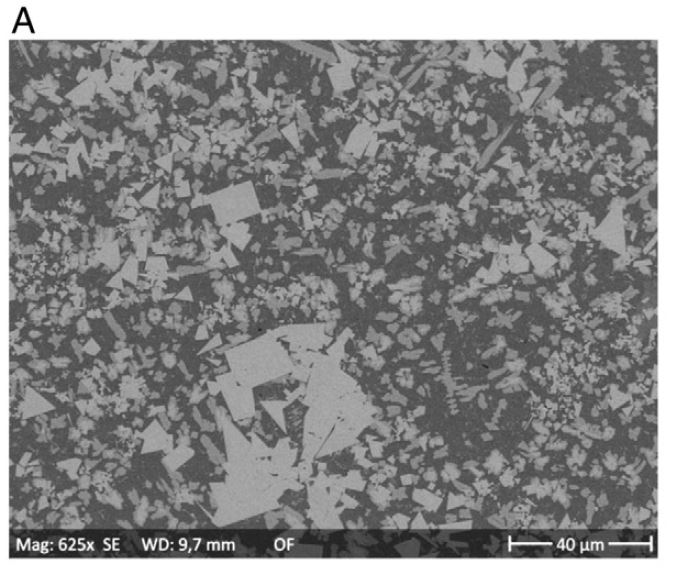
\includegraphics[scale=0.55]{images/срез1}
		\captionof{figure}{Микроструктура сплава WC–CoSi при низком разрешении}
		
		\end{minipage}
		\begin{minipage}{.49\textwidth}
	
			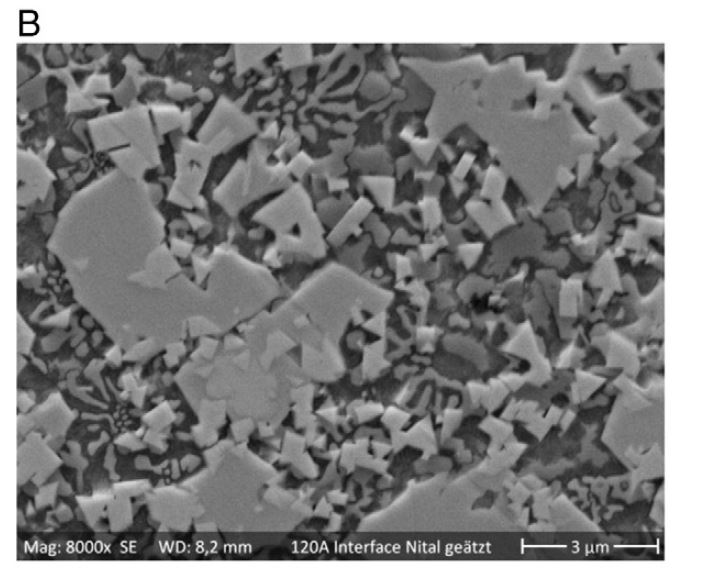
\includegraphics[scale=0.55]{images/срез2}
			\captionof{figure}{Микроструктура сплава WC–Co при при высоком разрешении}
		\end{minipage}
	
	\end{center}



	\begin{figure}[h!]
	\centering
	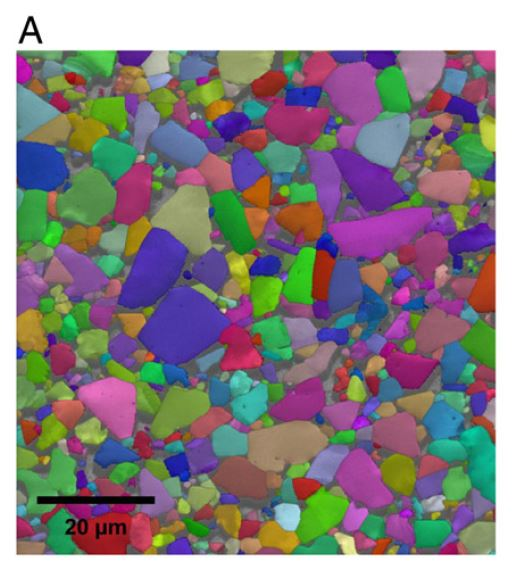
\includegraphics[scale=0.65]{images/зерна1}
	\caption{Микроструктура сементированного карбида с связующим веществом, EBSD}
	\end{figure}

	\section{Эксперименты и выводы}
	В данной работе износостойкость сплавов , содержищих цементированный карбид, 
    были измерены по стандартам
	ASTM B611 и ASTM G65-E.
	
	Износостойкость сверхшероховатых марок WC-Co резко
	повышается за счет нанозернистого армирования связующей фазы
	наночастицами со средним размером зерен почти 3 нм. 

	Износостойкость близких к наноразмерам цементированных карбидов несколько лучше,
	чем у соответствующих обычных связок WC-Co, только при
	относительно низком содержании Co.
	
	Близкие к наноуглеродам карбиды
	с высоким содержанием Co характеризуются более низким сочетанием твердости, износостойкости и
	трещиностойкости по сравнению с обычными связками WC.
	
	
	Средний размер зерен WC околонанокарбидов предположительно лежит
	выше гипотетической " пограничной линии”относительно возможности одновременного
	повышение как твердости, так и вязкости разрушения за счет
	наноструктурирования.
	
	

	
\end{document}